\subsection{Admin View}

%For the main pages put a mockup and describe it in detail.
\begin{center}
    \frame{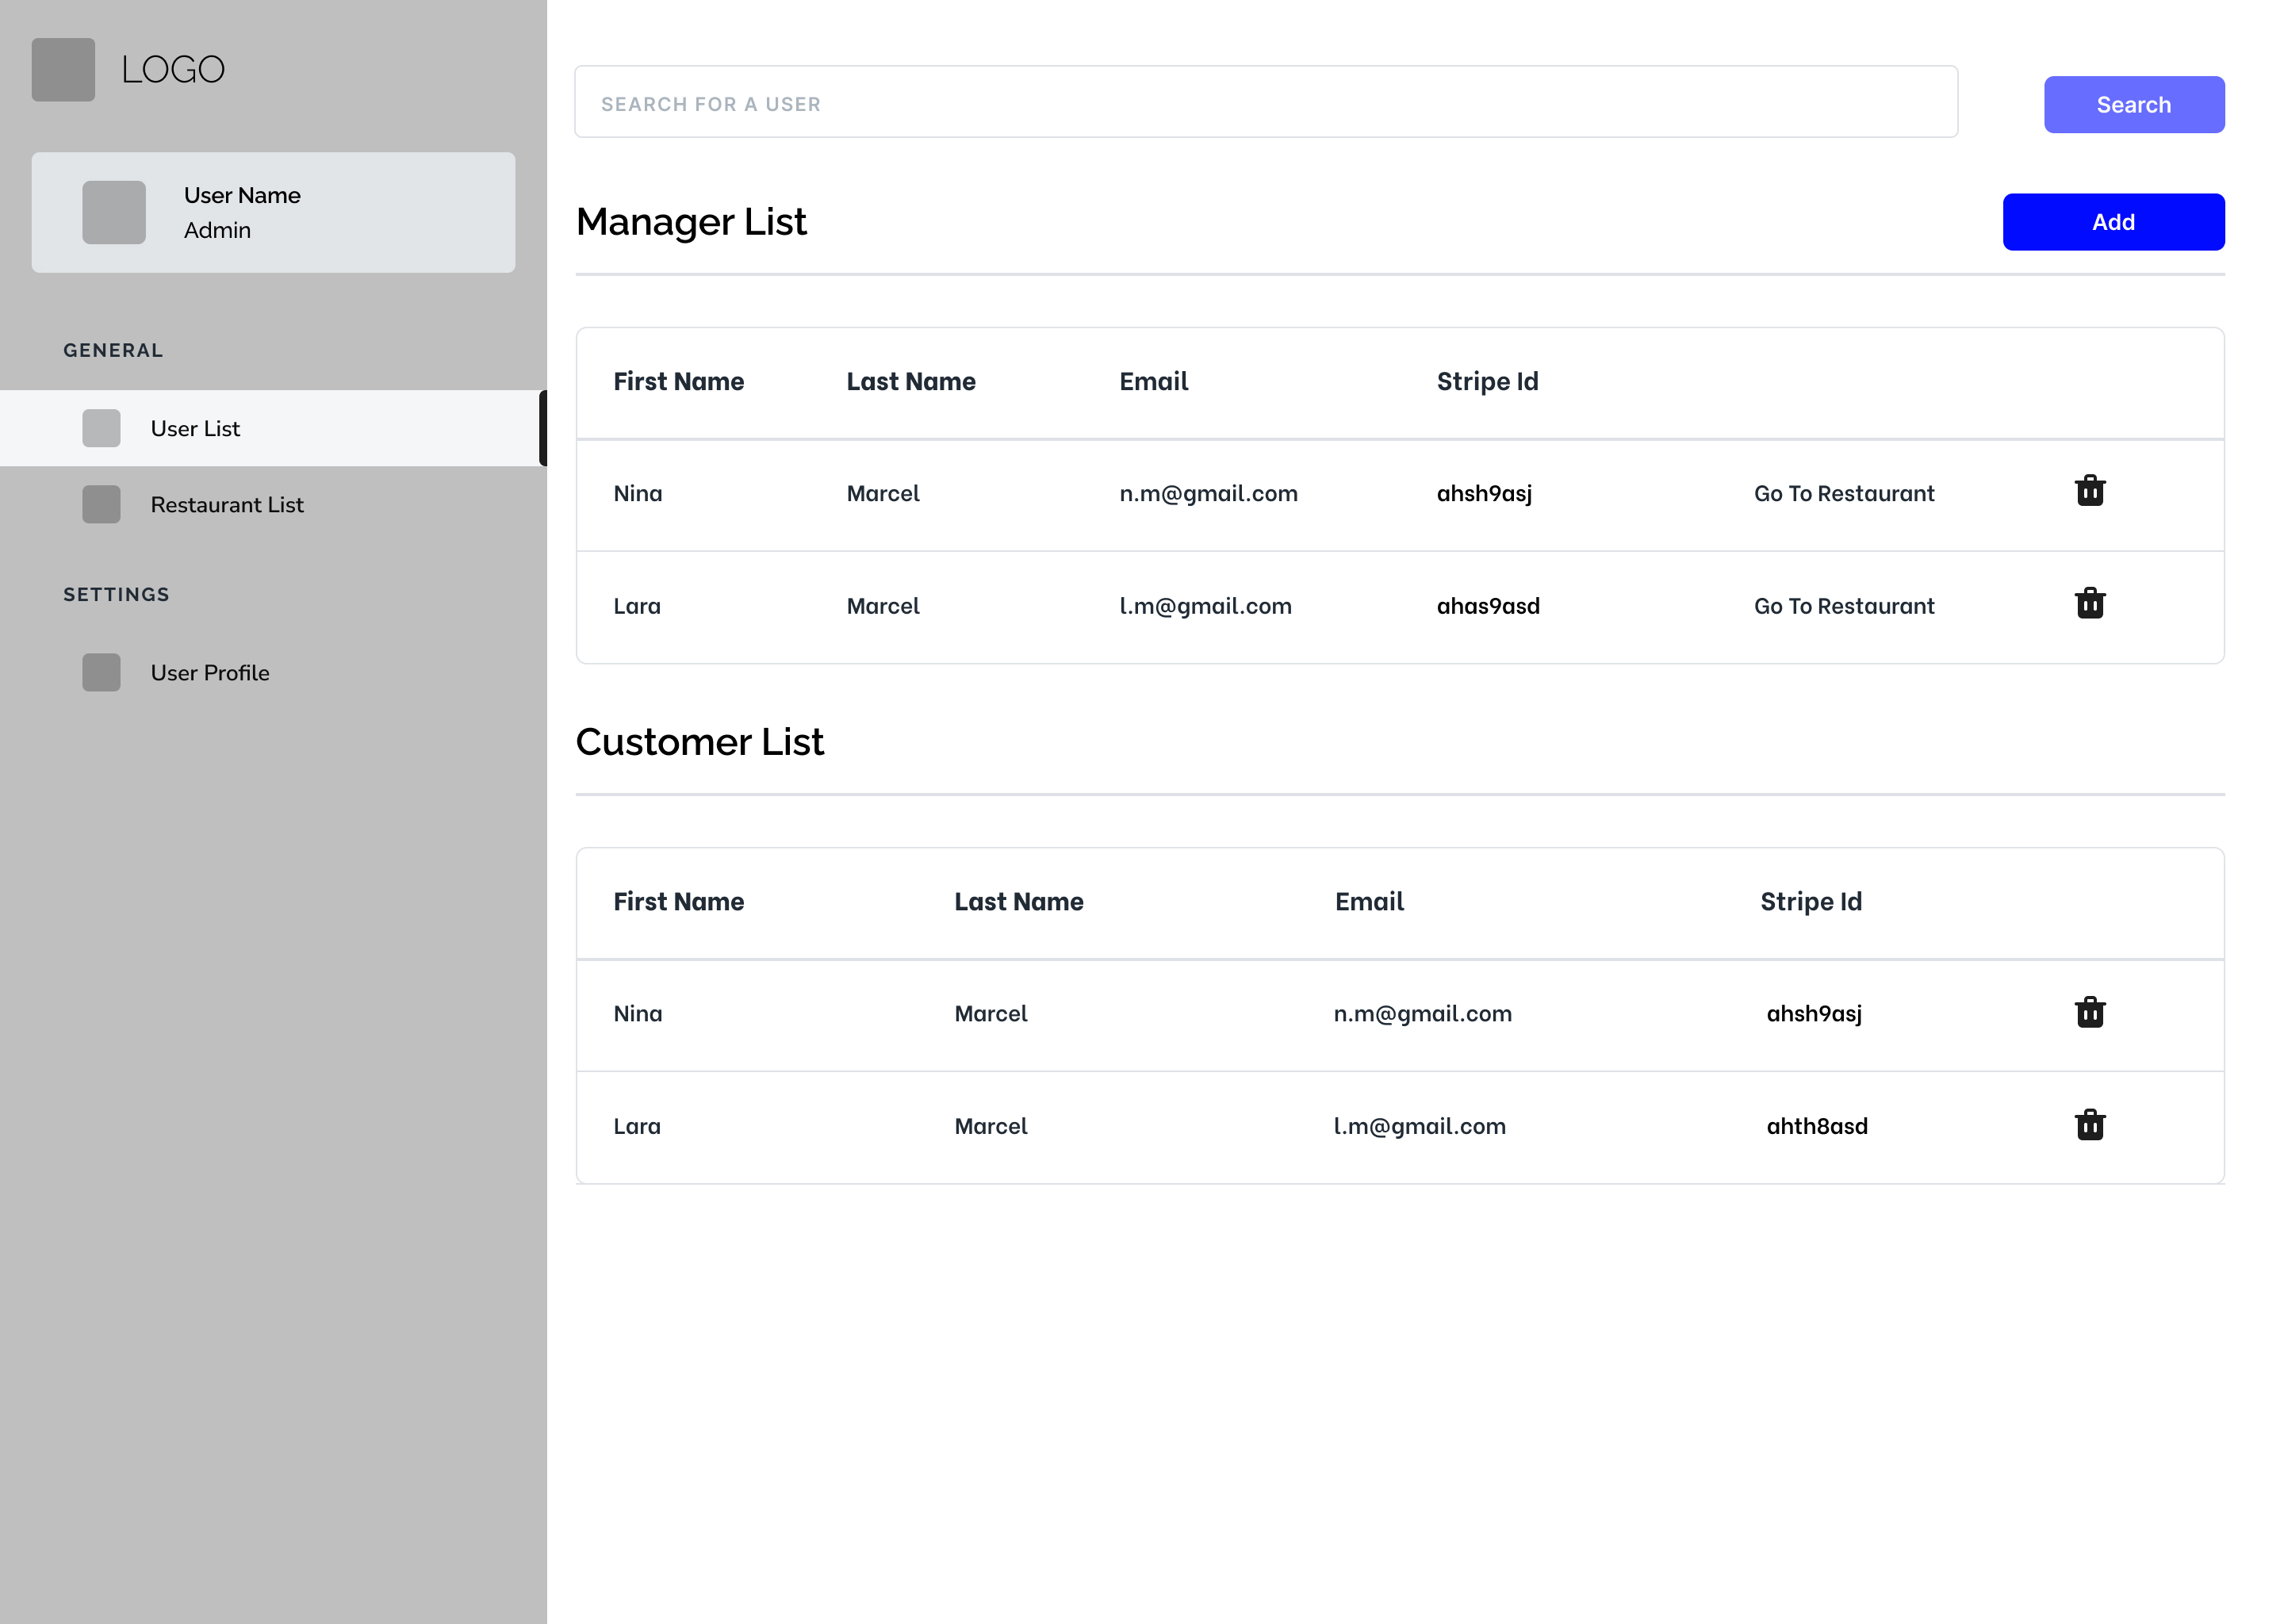
\includegraphics[width=.8\textwidth]{resources/mockup/admin/Admin-User-List.jpg}}
    \captionof{figure}{List of users from Admin view.}
    \label{fig:admin-ListOfUsers}
\end{center}

\begin{center}
    \frame{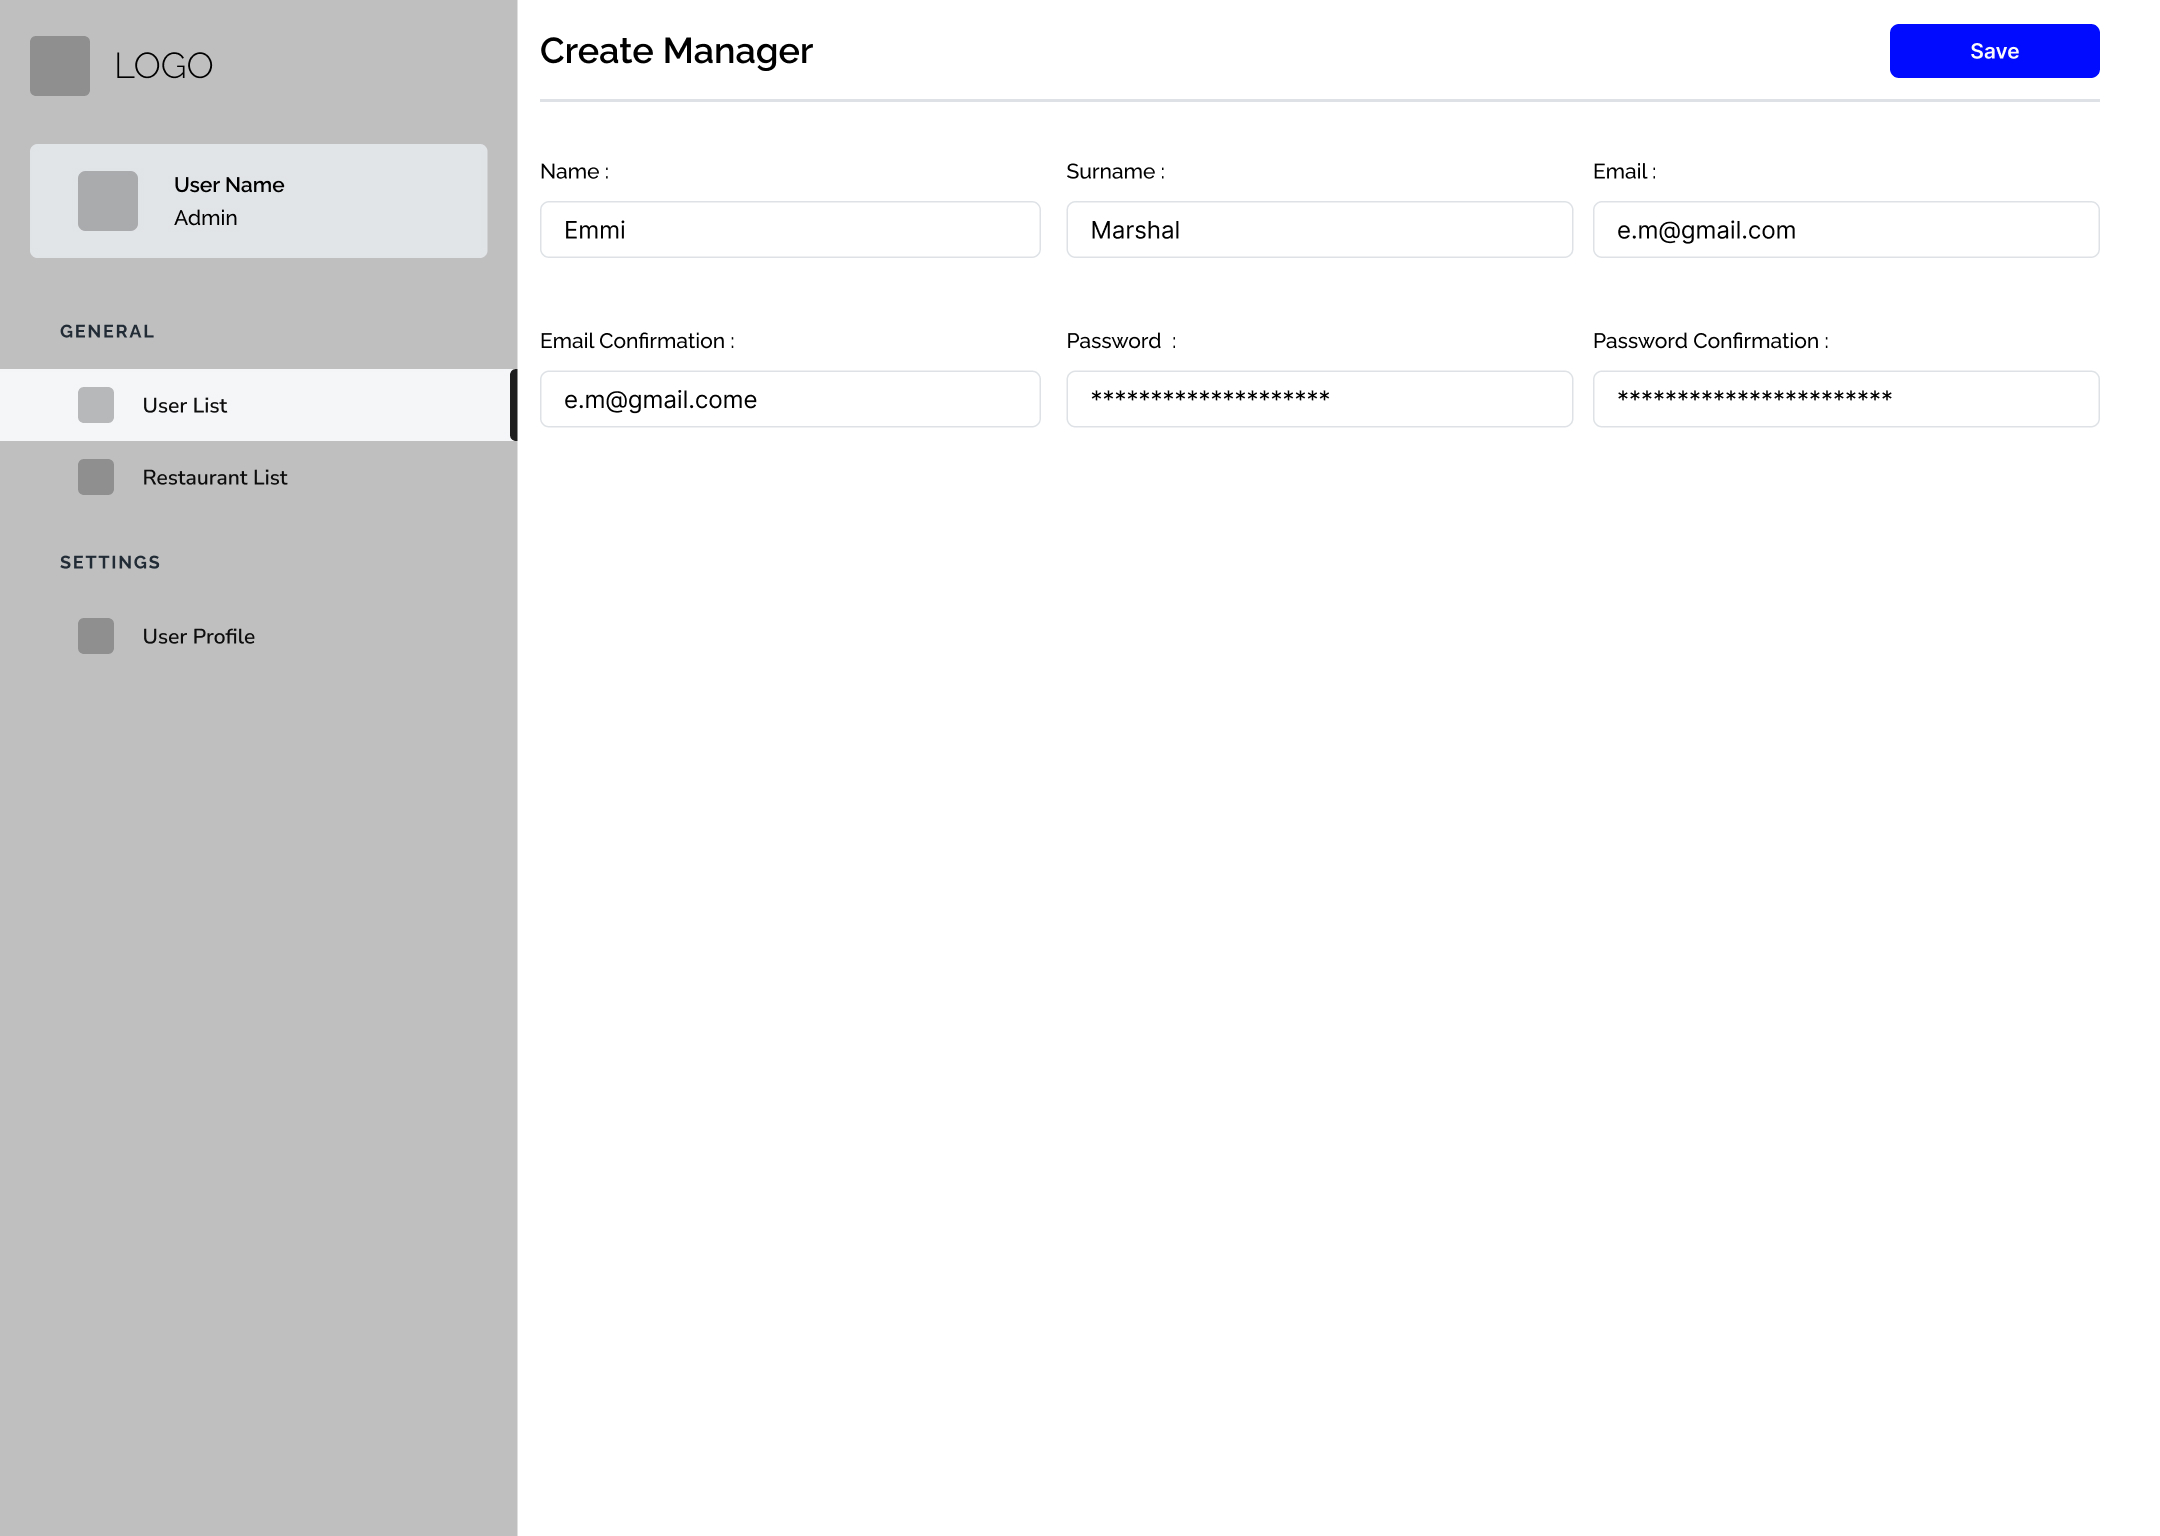
\includegraphics[width=.8\textwidth]{resources/mockup/admin/Admin-Create-Manager.jpg}}
    \captionof{figure}{Admin page for creating a new manager.}
    \label{fig:admin-CreateManager}
\end{center}

\begin{center}
    \frame{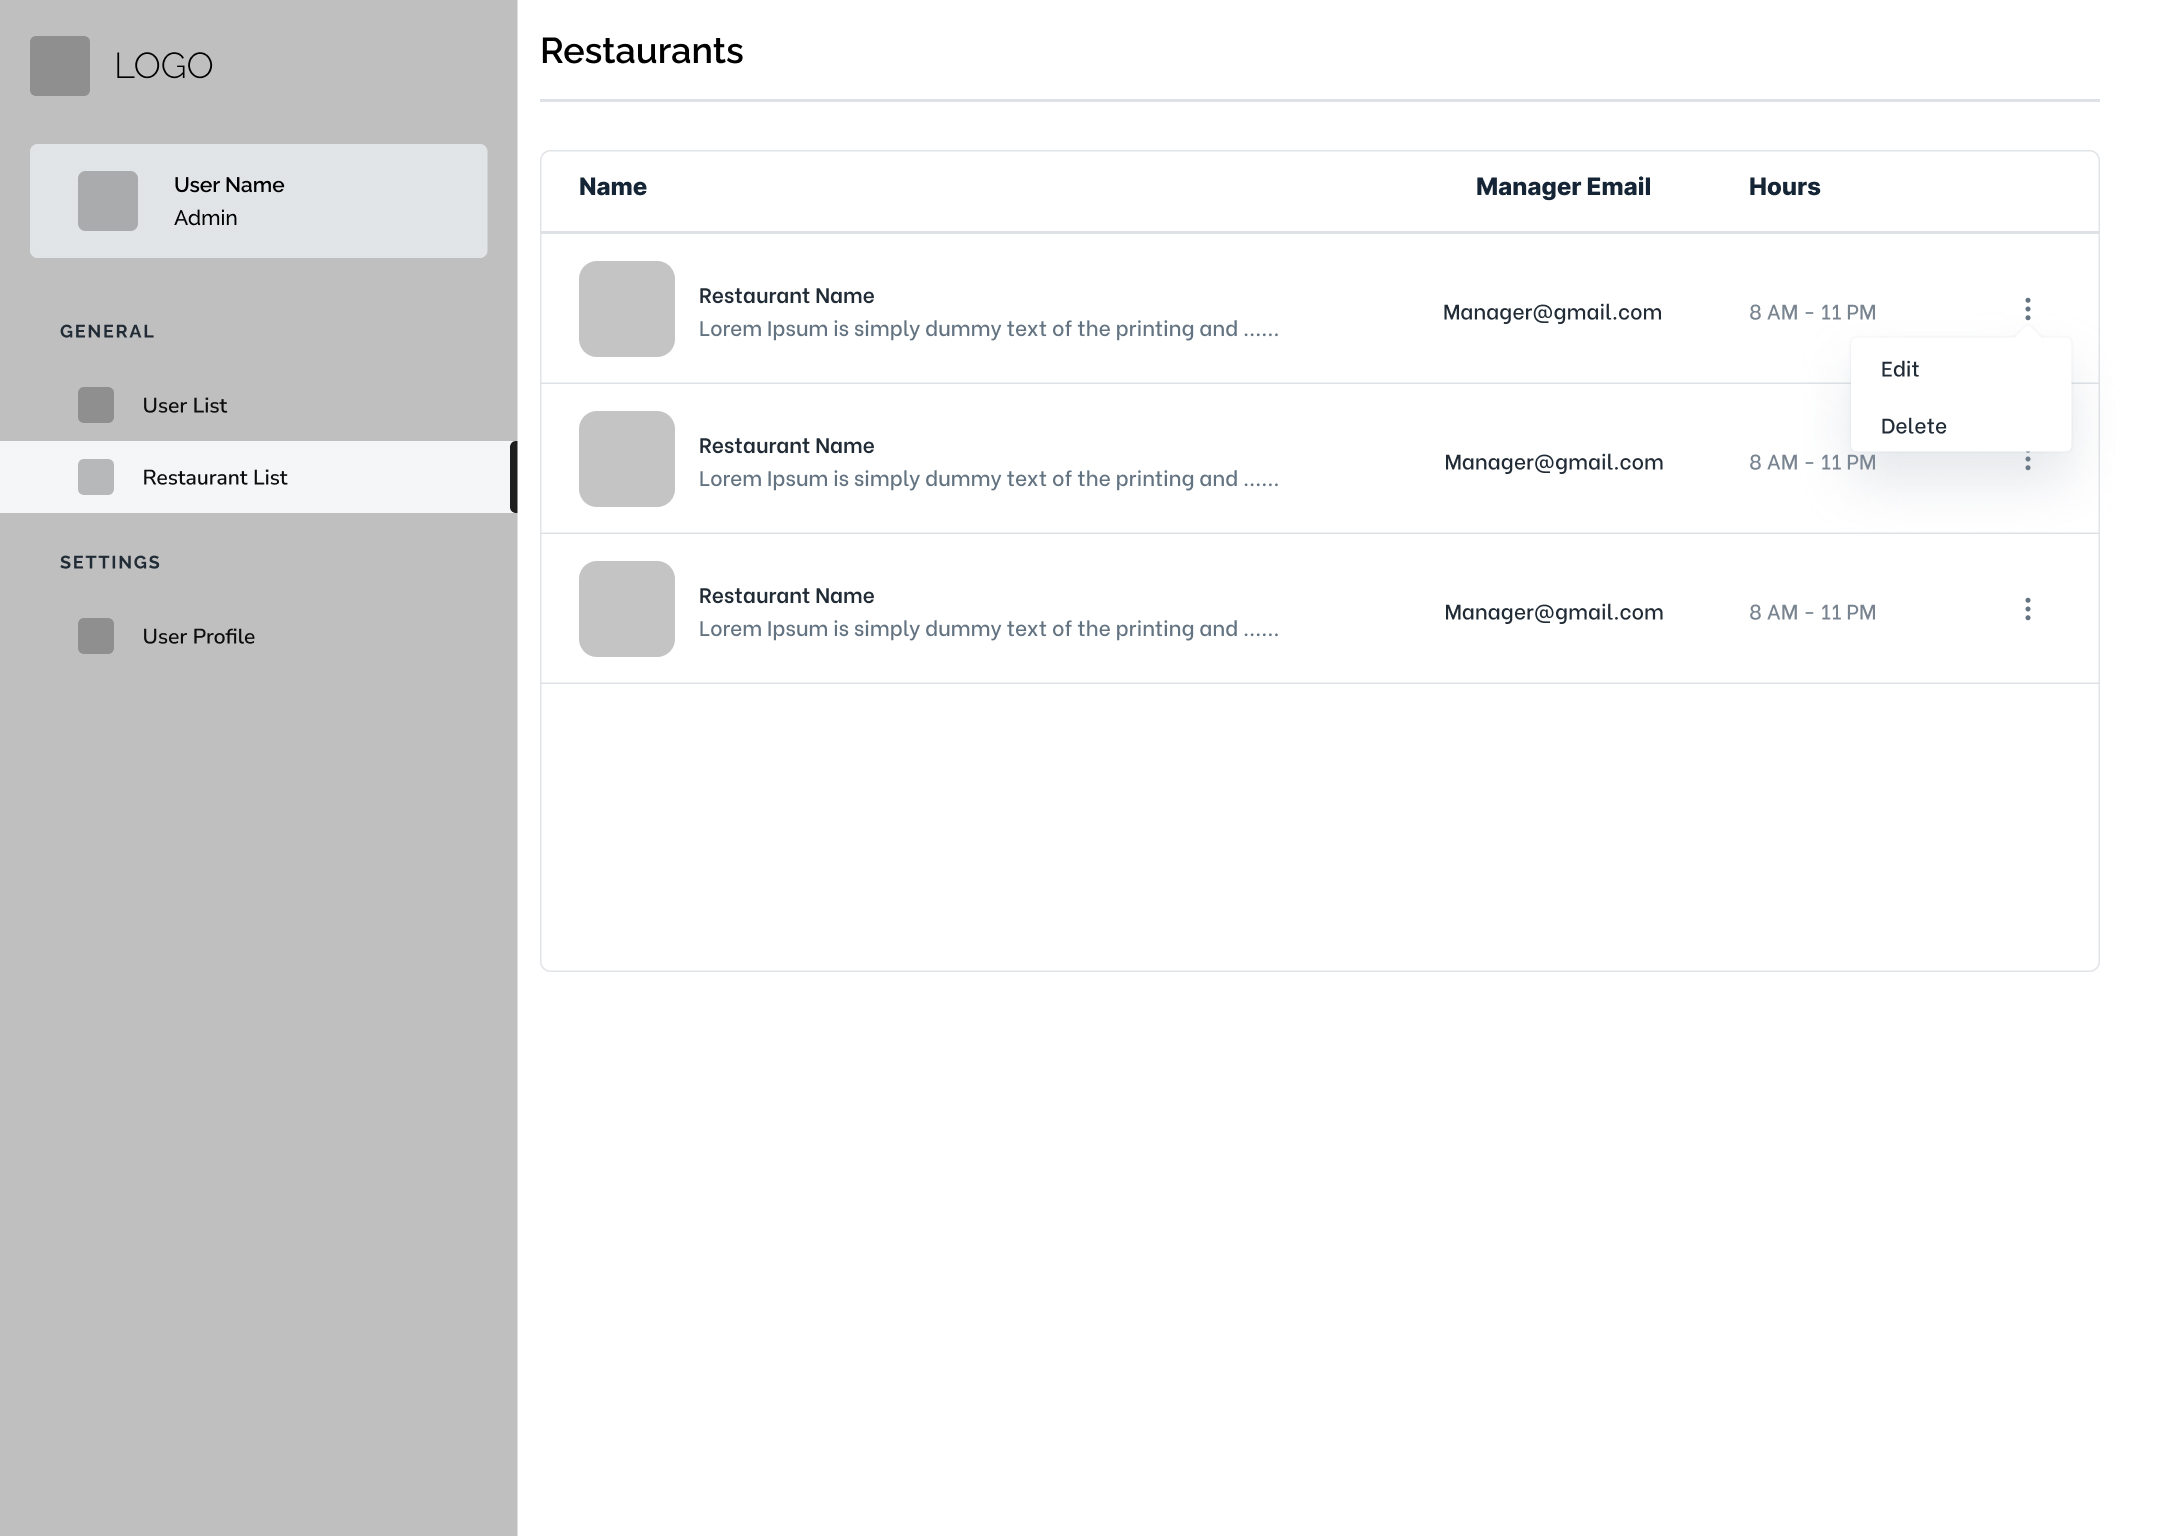
\includegraphics[width=.8\textwidth]{resources/mockup/admin/Admin-view-ListOfRestaurants.jpg}}
    \captionof{figure}{List of restaurants from Admin view.}
    \label{fig:admin-ListOfRestaurants}
\end{center}

\begin{center}
    \frame{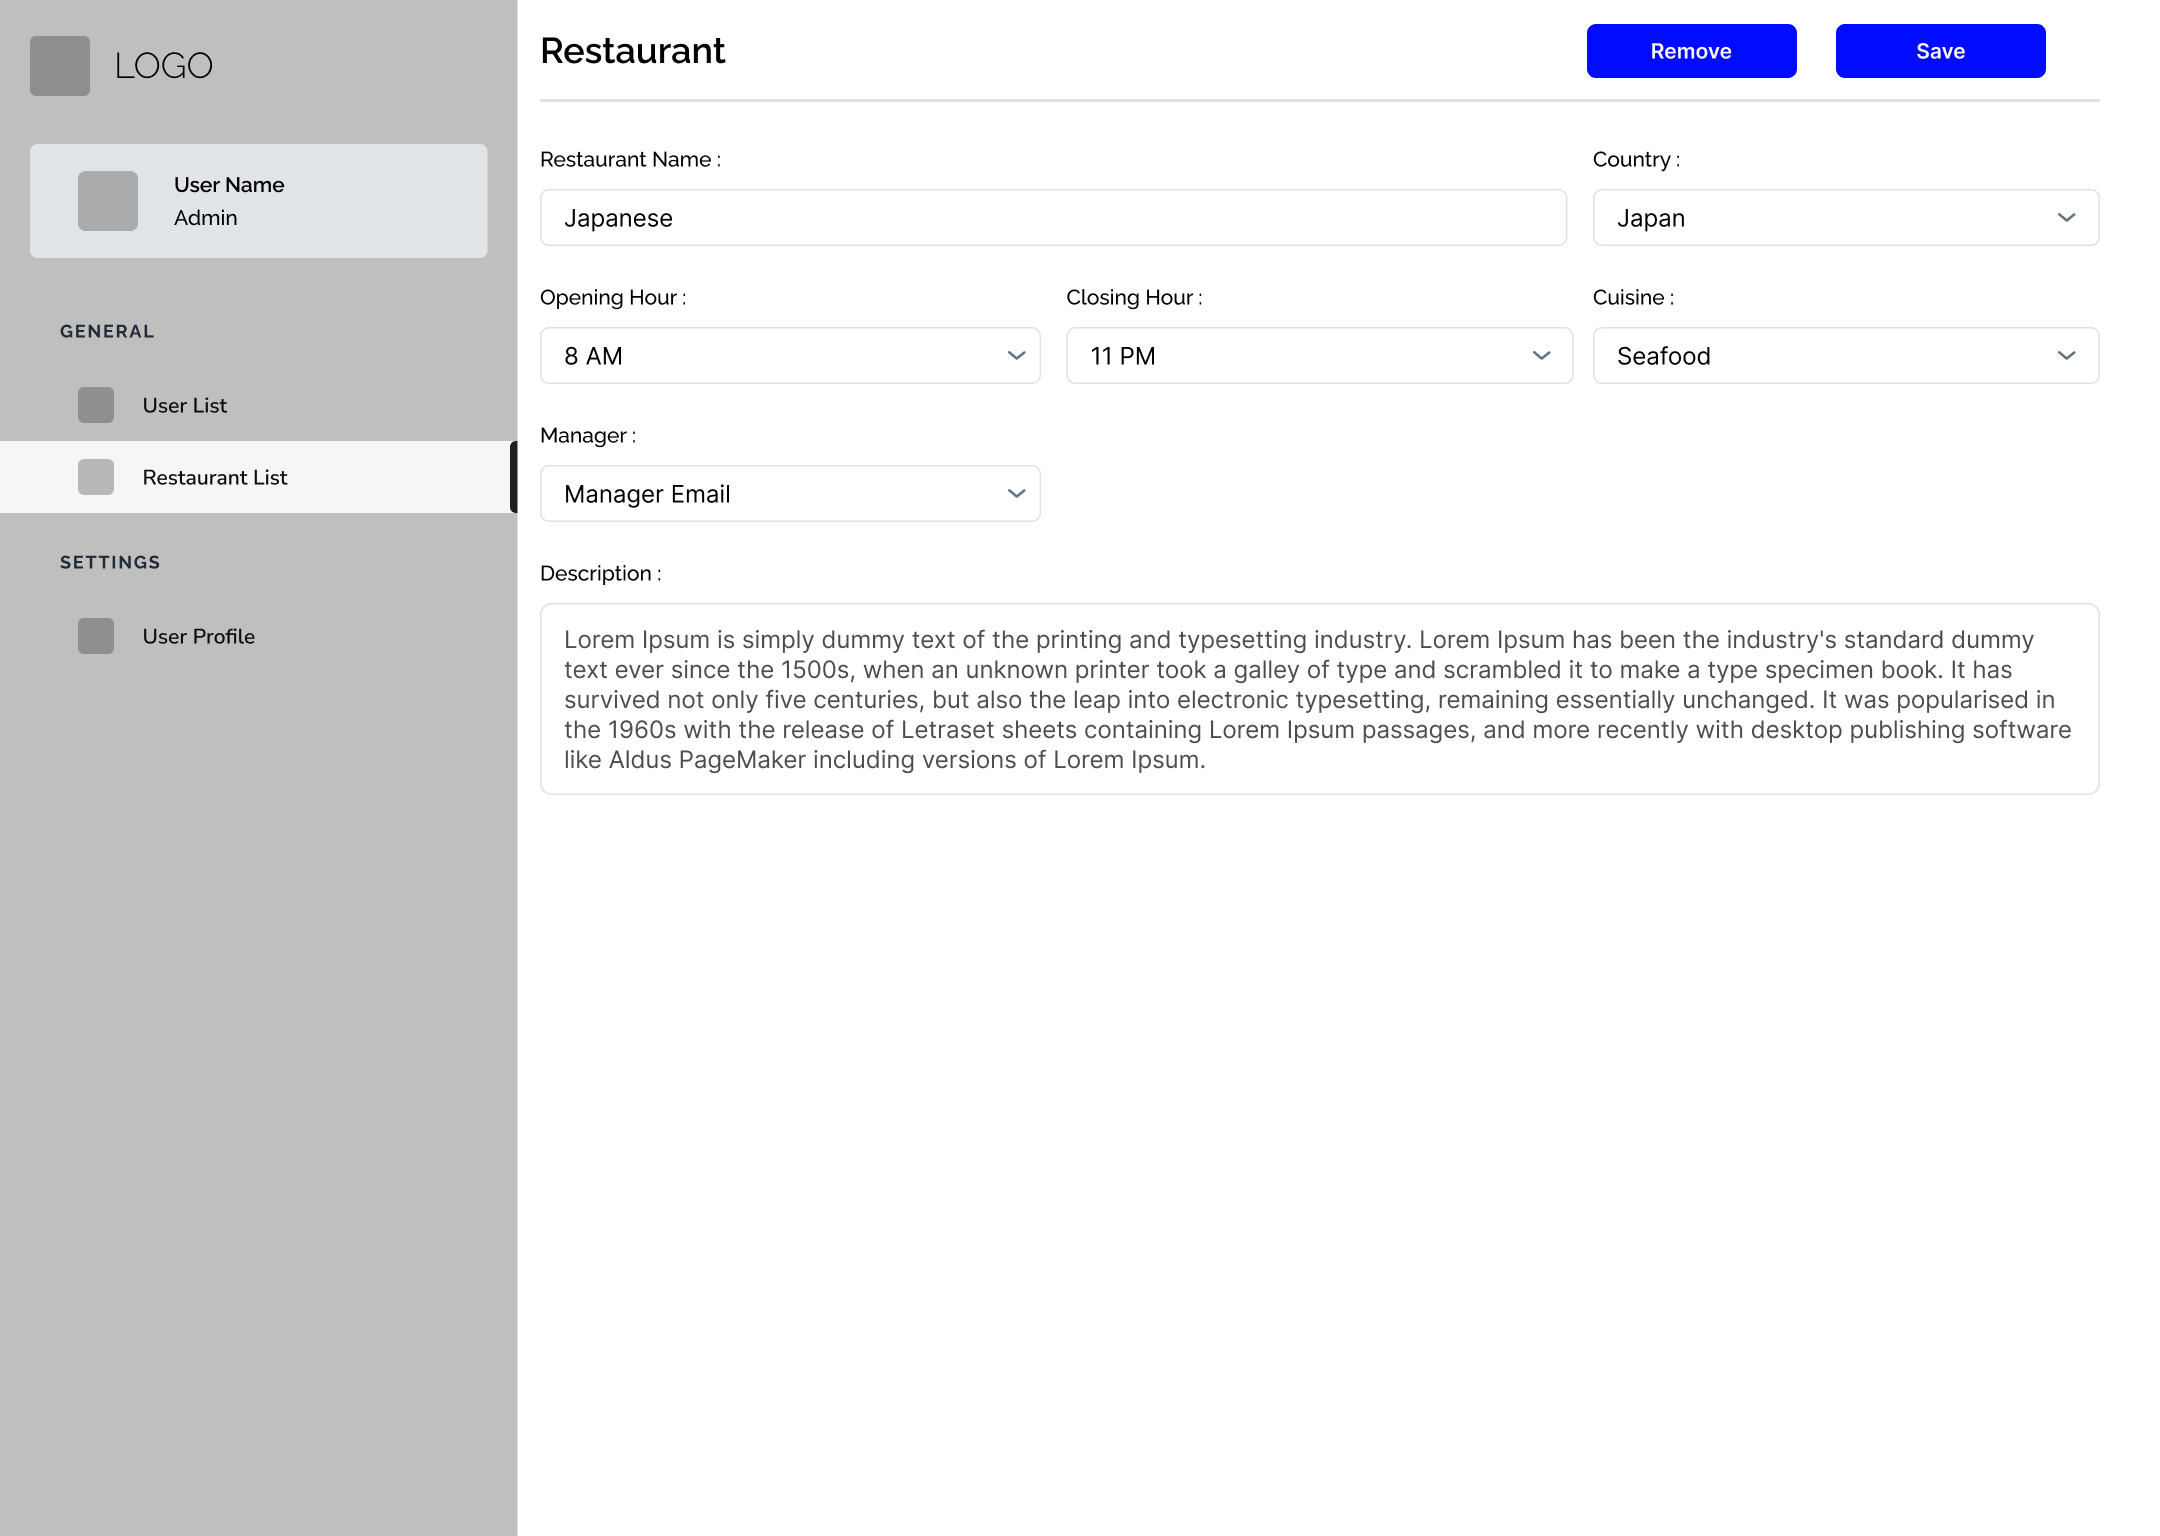
\includegraphics[width=.8\textwidth]{resources/mockup/admin/Admin-Edit-Restaurant.jpg}}
    \captionof{figure}{Restaurant editing page from Admin view.}
    \label{fig:admin-EditRestaurant}
\end{center}

The list of users, Figure \ref{fig:admin-ListOfUsers}, can be seen only by the admin, who can remove users or add a new manager.
We set a specific page for creating a new manager, Figure \ref{fig:admin-CreateManager}, accessible only by the admin, because, prior to creation, the admin and the new manager should have met and discussed about the possibility of bringing the manager's restaurant(s) to the festival. The admin can also see the list of all restaurants or the one(s) associated to a specific manager, Figure \ref{fig:admin-ListOfRestaurants}, and can also edit the restaurant info, because at some point a restaurant could be changing the manager and the admin is the one that can edit the manager field on each restaurant, as shown in Figure \ref{fig:admin-EditRestaurant}.